%===================================== CHAP 5 =================================

\chapter{Analysis}

As explained in section \ref{section:differential_privacy}, differential privacy works by disguising an individual's data in a dataset by adding noise to their records. The amount of noise added is determined by the privacy parameter  $\epsilon$, and grows exponentially the closer the parameter gets to zero. 

\begin{figure}[h!]
	\centering
	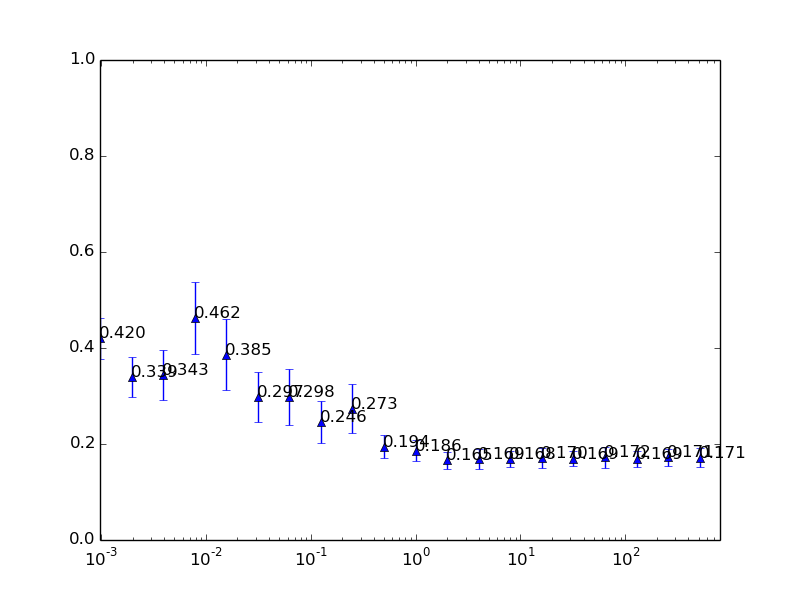
\includegraphics[width=\textwidth]{fig/eps2e-10-2e9,bud=eps,peers50,groups50,reg2e-4}
 	\caption{$\epsilon = [2^{-10}, 2^{9}], \lambda = 2^{-4}$, 50 peers, 1 aggregation}
 	\label{fig:epsilon_big_range}
\end{figure}
 
Figure \ref{fig:epsilon_big_range} shows the effect of the privacy parameter $\epsilon$ in our experiment. We wanted to test the effect of varying the $\epsilon$-value in the range from $2^-10$ to $2^9$, especially to find out how the classifier would perform when faced with data with high amount of noise added to it. 
 
\begin{figure}[h!]
	\centering
	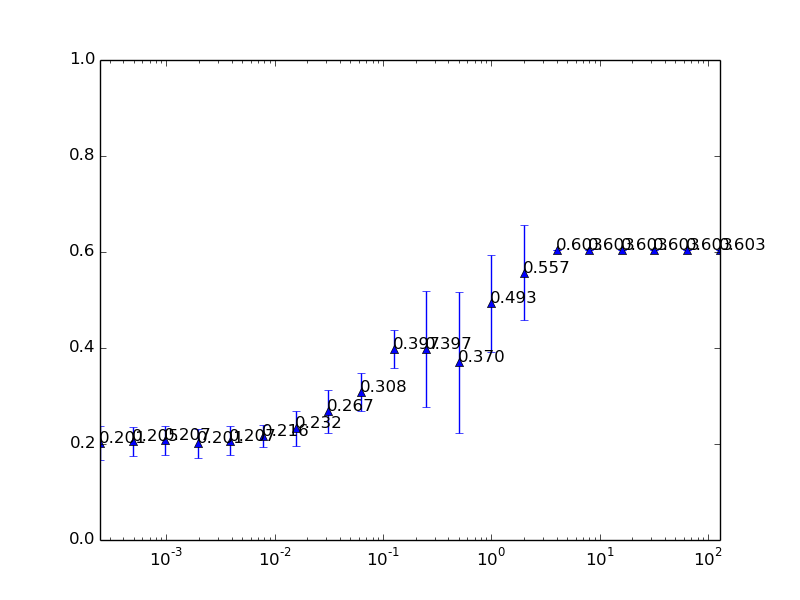
\includegraphics[width=\textwidth]{fig/eps2e10.0,bud2e10.0,peers10,groups5,reg2e-12-2e7}
	\caption{$\epsilon = 2^{10}, \lambda = [2^{-12}, 2^{7}]$, 50 peers, 1 aggregation}
	\label{fig:regularization_extremelyhighepsilon}
\end{figure}

Figure \ref{fig:regularization_extremelyhighepsilon} shows the normal effect regularization has on accuracy. As the regularization parameter $\lambda$ grows large, the model becomes less able to fit the training data, eventually resulting in models predicting only the negative class. On this particular dataset it appears that a logistic regression model is not at risk of overfitting, since the cross validated error does not increase when the level of regularization is very low. In a context where privacy is irrelevant, this would mean that selecting some regularization parameter in the range $[10^{-5},10^{-2}]$ could be acceptable. Choosing a level at the high end of this range could be a good idea, to reduce the risk of overfitting.

When noise, tuned to offer $epsilon$-differential privacy, is added to the model creation process, the trade-offs involved in choosing regularization $\lambda$ become more tricky.

What are the results of our experiments?

What did we learn from the basic structure of creating our framework?

What difficulties did we encounter?

What can we take away from our experiments?

What should have been done better? 

What did we learn from tuning the different parameters?

More data per peer leads to better classification. With small number of peers, there are more records per peer. This generally leads to better classification accuracy. Why is this? 

Australian: Sweet spot for regularization at a 2e-3, 10 peers 5 groupsize

What was the effect of tuning the regularization parameter? High and low regularization leads to more SD on the error rate, but there is a sweet spot.

What was the effect of increasing the epsilon? 
	It seemed like it was better to keep the perUpdateBudget smaller than the epsilon, so that the models are aggregated more. Did this lead to better accuracy? Why do more aggregations lead to better classification than having a bigger budget but only one aggregation.
	
Compare the results of our distributed logistic regression classifier with the tradional ones in literature. Sharma and Arora \cite{sharma2013adaptive} report getting 92.95\% classification accuracy on the same data set. Kumar et al\cite{kumar2012comparative}. reports  0.1389 error rate before filtering when using logistic regression combined with a least squares regularization method. Our classifier can compare to these under certain circumstances, even after noise addition.  



\section{Potential Future applications}
This section will discuss the potential application of a system based on our distributed machine learner.

\subsection{Health}
A growing worldwide market is the sale and usage of wearable sensors, such as environmental sensors, motion sensors, and health sensors. A IHS report \cite{ihs2014reportwearables} from 2014 estimates that the market for sensors in wearables will expand to 135 million units in 2019, up from 50 million in 2013. These wearables will evolve from being just a single purpose device such as a pedometer and grow into more multipurpose devices such as a smartwatch, which will consist of several sensors which can monitor several components within its area of use. 

The wearable devices are implementing fitness and health monitoring by using a mixture of sensors, such as motion, pulse, hydration and skin temperature sensors. All of these wearables will therefore generate a massive amount of data about the person who are using them. This data can be considered as highly sensitive information, as it can unveil a lot about their user's health, and the manufacturers of these devices knows this. Dana Liebelson, a reporter for Huffington Post, queried several US-based fitness device companies about their privacy. One of the replies she got, was that "the company does not sell information collected from the device that can identify individual users", but that they were considering marketing aggregate information that cannot be linked back to an individual. As we saw in section \ref{section:privacy_breaches} and \ref{section:attack_vectors}, many of the popular methods for aggregating and anonymizing a dataset carries an inherent risk of a privacy breach.



-Future homes can potentially track you through you phone, or similar device. 

-You don't want to send this data to someone else, but what you can learn from the data can be highly useful in your daily life. 

Kevin Fong and the England rugby team. Monitor heart rate, step balance, and a lot of other factors. Can pick up injuries and illnesses well before any doctor. This will trickle down into daily use over the next decade. 


\cleardoublepage